\documentclass[12pt]{article}
\usepackage{sbc-template}
\usepackage{graphicx,url}
\usepackage[brazil]{babel} 
\usepackage[utf8]{inputenc}
\usepackage{placeins}
\usepackage{longtable}
\usepackage{multirow}

\sloppy

\title{Plano de gerenciamento de riscos:\\Site de venda de ingressos}

\author{
    \begin{minipage}{\textwidth}
        Carlos Alberto\inst{1},
        Daniela Menezes\inst{2},
        Danilo Caldeira\inst{3},
        Gabriel Augusto R. dos Reis\inst{4},
        Giovani Araújo\inst{5},
        Guilherme Ferreira Faioli Lima\inst{6},
        Indianara Santos Rodrigues\inst{7},
        Luiz Carlos Silva Júnior\inst{8}
    \end{minipage}
}
\address{
    Departamento de Computação e Sistemas\\
    Universidade Federal de Ouro Preto (UFOP) -- João Monlevade, MG\\
    \\16.2.8394 \inst{1}, 
    16.2.8540 \inst{2},
    16.2.8512 \inst{3},
    16.2.8105 \inst{4},
    16.2.8149 \inst{5},
    16.1.8243 \inst{6},
    17.2.8246 \inst{7},\\
    15.1.5881 \inst{8}
}

\begin{document}

    \maketitle

    \begin{abstract}
        This management plan aims to identify all risks associated with the project, as well as understand them in order to avoid them and in case they occur to know how to correct the failure. The identification and evaluation of these risks will be carried out in a brainstorming, in addition to using SWOT analysis, detailed in figure \ref{fig:swot}, as well as checklists and lessons learned from previous projects.
    \end{abstract}

    \begin{resumo}
        Este plano de gerenciamento tem como objetivo identificar todos os riscos associados ao projeto, assim como entendê-los afim de evitá-los e caso eles ocorram saber como corrigir a falha. A identificação e avaliação desses riscos serão realizadas em um brainstorming, além de utilizar a análise SWOT, detalhada na figura \ref{fig:swot}, assim como checklists e as lições aprendidas com projetos anteriores.
    \end{resumo}
    
\tableofcontents
\newpage

    \begin{figure}[ht]
        \centering
        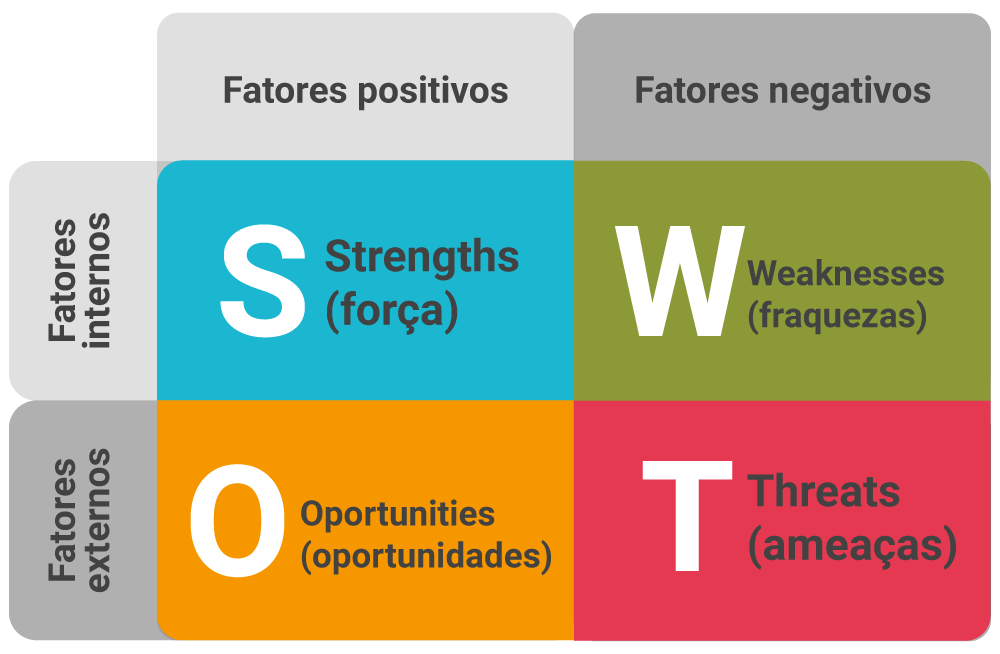
\includegraphics[scale=0.3]{./Images/swot.png}
        \caption{Gráfico SWOT}
        \label{fig:swot}
    \end{figure}

    \section{Identificar riscos associados ao projeto}
        \begin{itemize}
            \item Perda de dados.
            \item Layout ruim.
            \item Usabilidade confusa.
            \item Repostas erradas do Banco de dados.
            \item Erros de sincronização com os métodos de pagamento.
            \item Erros associados ao mecanismo de busca.
            \item Erros com editor de conteúdo.
            \item Erros relacionados a portabilidade.
            \item Número de usuários maior que o planejado.
            \item Usuários resistentes ao sistema.
            \item Ataque Hacker.
            \item Marketing ruim do site.
            \item Risco financeiro.
            \item Falta de atualização dos cinemas ou sessões.
            \item Preços não competitivos no mercado ou com o próprio cinema localmente.
            \item Satisfação do cliente. 
            \item Inutilização dos cinemas.
        \end{itemize} 
        
    \section{Avaliar probabilidade de ocorrência}
        De acordo com a Figura \ref{fig:swot}, os riscos identificados serão qualificados de acordo com sua probabilidade de ocorrência.
        
        \begin{itemize}
            \item  Probabilidade:
            \begin{itemize}
                \item Baixa - A probabilidade de ocorrência do risco pode ser considerada pequena.               
                \item Média - Existe uma probabilidade razoável de ocorrer o risco.
                \item Alta - O risco é iminente.
            \end{itemize}
            \item Gravidade:
            \begin{itemize}
                \item Baixa - O impacto do evento de risco é irrelevante, tanto em termos de custo, prazo, podendo ser resolvido facilmente.
                \item Média - O impacto de evento de risco é relevante e necessita de gerenciamento mais preciso.
                \item Alta - O impacto do evento de risco é elevado e, caso não haja uma interferência imediata e precisa, os resultados serão comprometidos.
            \end{itemize}
        \end{itemize}
       
        \begin{table}[h]
            \centering
            \label{table:gravidade_e_riscos}
            \resizebox{\textwidth}{!}{
                \begin{tabular}{|l|c|c|}
                    \hline
                    \multicolumn{1}{|c|}{\textbf{Riscos}} & 
                    \multicolumn{1}{|c|}{\textbf{Probabilidade}} & 
                    \multicolumn{1}{|c|}{\textbf{Gravidade}} \\ \hline
                    Perda de dados & baixa & alta \\ \hline
                    Layout ruim & baixa & baixa \\ \hline
                    Usabilidade confusa & baixa & média \\ \hline
                    Repostas erradas do Banco de dados & baixa & alta \\ \hline
                    Métodos de pagamento & baixa & alta \\ \hline
                    Mecanismo de busca & média & baixa \\ \hline
                    Portabilidade & média & alta \\ \hline
                    Número de usuários maior que o planejado & baixa & baixa \\ \hline
                    Ataque Hacker & média & alta \\ \hline
                    Marketing ruim do site & média & baixa \\ \hline
                    Risco financeiro & baixa & alta \\ \hline
                    Falta de atualização dos cinemas ou sessões & alta & alta \\ \hline
                    Preços não competitivos no mercado ou com o próprio cinema localmente & alta & alta \\ \hline
                    Satisfação do cliente & baixa & média \\ \hline
                    Inutilização dos cinemas & baixa & alta \\ \hline
                \end{tabular}
            }
            \caption{Probabilidade e gravidade dos riscos}
        \end{table}
    \FloatBarrier

    \section{Estimar impacto}

        \begin{center}
            \begin{longtable}{|p{2.0cm}|p{3.2cm}|c|p{3.2cm}|c|}
                
            
                \hline 
                \multicolumn{1}{|c|}{\textbf{Riscos}} & 
                \multicolumn{1}{c|}{\textbf{Descrição}} & 
                \multicolumn{1}{c|}{\textbf{Probabilidade}} &
                \multicolumn{1}{c|}{\textbf{Impacto}} &
                \multicolumn{1}{c|}{\textbf{Gravidade}} \\ \hline 
                \endfirsthead

                \multicolumn{5}{c}%
                {{\bfseries \tablename\ \thetable{} -- continuação da última página}} \\
                \hline 
                \multicolumn{1}{|c|}{\textbf{Riscos}} & 
                \multicolumn{1}{c|}{\textbf{Descrição}} & 
                \multicolumn{1}{c|}{\textbf{Probabilidade}} &
                \multicolumn{1}{c|}{\textbf{Impacto}} &
                \multicolumn{1}{c|}{\textbf{Gravidade}}\\ 
                \endhead

                \hline 
                \multicolumn{5}{|r|}{{Continua na próxima página}} \\ \hline
                \endfoot

                \hline \hline
                \endlastfoot
                
                Perda de dados & Devido a problemas no banco de dados, os dados podem ser momentaneamente perdidos & baixa & O software pode ficar inoperante até que o problema seja resolvido. & alta \\ \hline
                
                Layout ruim & Caso o site não funcione corretamente não irá proporcionar uma experiência agradável ao usuário  & baixa  & Perda de usuários e consequentemente perda de lucro & baixa  \\ \hline
                
                Usabilidade confusa & Uma navegação complexa pode fazer com que o visitante abandone o site. & baixa  & Perda de visitantes & média \\ \hline
                
                Repostas erradas do Banco de dados & Banco de dados retornam ingressos ou dados relativos ao ingressos ou sessões de forma errada & baixa & Gera compras erradas, inesperadas ou inexistentes, causando transtorno aos clientes, prejuízo ao site e má reputação perante os clientes & alta  \\ \hline
                
                Métodos de pagamento & Método de pagamento para de responder como o esperado, deixando de efetuar ou confirmar as transações & baixa & Parada nas vendas, gerando prejuízos até que o sistema retorne ao normal & alta  \\ \hline
                
                Mecanismo de busca & Campos de busca são áreas bastante utilizadas para encontrar o conteúdo do site o mais rápido possível. & média  & Visitante frustrado e consequentemente perda de visitantes  & baixa  \\ \hline
                
                Portabilidade & Site funciona de forma inesperada em browsers ou dispositivos diferentes & média & Usabilidade ruim do site & alta \\ \hline
                
                Número de usuários maior que o planejado & Número de usuários acessando simultaneamente o site é maior que o esperado & baixa & Clientes ativos não terão problemas, a medida que os novos visitantes não conseguirão acessar até que um antigo saia e libere o recurso & baixa \\ \hline
                
                Ataque Hacker & Devido a uma falha de segurança em qualquer parte da infraestrutura, uma pessoa mal-intencionada, pode invadir o servidor e ter acesso a dados privados, podendo alterá-los ou divulgá-los de forma indevida. & média & A empresa pode sofrer processos legais caso os dados privados sejam descobertos ou o site pode ficar temporariamente inoperante. & alta \\ \hline 
                
                Marketing ruim do site & divulgação de forma errada, sem alcance ou desinteressante aos possíveis clientes & média & Desinteresse de novos clientes & baixa  \\ \hline
                
                Risco financeiro & Incerteza sobre futuro financeiro da empresa & baixa & Revisão nos planos da empresa & alta  \\ \hline 
                
                Falta de atualização dos cinemas ou sessões & Não atualizar os dados dos cinemas ou sessões de filmes & alta & Compras erradas ou falta de opções de compra & alta  \\ \hline 
                
                Preços não competitivos no mercado ou com o próprio cinema localmente & Preços mais caros ou não vantajosos quando comparado com concorrentes ou o próprio cinema & alta & Não serão realizadas novas vendas & alta  \\ \hline 
                
                Satisfação do cliente & reclamações sobre o site, principalmente nas redes sociais & baixa & danos à identidade digital & média  \\ \hline 
                
                Inutilização dos cinemas & Tecnologia ficar ultrapassada ou ser substituída & baixa & Adequação ao novo mercado ou tecnologia & alta  \\ \hline 
              
                \caption{Descrição dos riscos e seus Impactos}
                \label{Descricao_E_Impacto_Dos_Riscos}
            \end{longtable}
        \end{center}

        
    \subsection{Estabelecer plano de contingência}
       
       \begin{itemize}
       \item Perda de dados: A melhor forma de evitar a perda de dados é fazer backups periódicos ou sistemas distribuídos.
       
       \item  Layout ruim: Para que o site funcione corretamente e proporcione uma experiência agradável ao usuário é necessário que a parte visual/estética estejam alinhados. Caso haja exagero nas cores, tamanho de imagem inadequado que atrapalhe a qualidade visual da tela é necessário que o layout seja refeito.
       
        \item Usabilidade confusa: É necessário que parte do site seja refeito de maneira simples, inidentificável e direta, seguindo o padrão na construção das páginas, agrupar o conteúdo do site em categorias lógicas fazendo com que a resposta por uma procura seja mais direta possível.
        
        \item Respostas erradas do banco de dados: Caso seja identificado um método de pequisa que gere uma resposta errada, um desenvolvedor de manutenção do software deve ser chamado para que posso ser analisado o motivo do erro e então liberada uma versão de correção do software o mais rápido possível.
        
        \item Métodos de pagamento: Contactar imediatamente a empresa terceirizada responsável pelo pagamento para que seja reparado ou se necessário, efetuar a troca da empresa terceirizada.
       
        \item Mecanismo de busca: Caso as buscas gerem resultados inesperados, as consultas feitas no banco de dados devem ser repensadas para que os erros não se repitam.
        
        \item Portabilidade: Caso seja identificado um dispositivo ou browser que gere um layout     método de pequisa que gere um layout "quebrado", deve-se verificar quais as características do dispositivo para que possa ser corrigido e então liberar uma versão de correção do software o mais rápido possível.
        
        \item Número de usuários maior  que o planejado: Caso o site não suporte a quantidade de usuários, será necessário aumentar a capacidade do servidor.
        
        \item  Ataque Hacker: Verificar em qual área o ataque foi feito, caso sejam dados privados, alertar a todos os envolvidos imediatamente, caso dados sejam modificados, o backup deverá ser consultado e restaurado, caso contrário reestabelecer o servidor para que o site volte a operar normalmente.
        
        \item Marketing ruim do site: Após verificar a efetividade do marketing atual (cruto, médio e longo prazo), refazer todo o conceito de divulgação do site.
        
        \item Risco financeiro:  Revisão constante das finanças e planejamento financeiro futuro detalhado e discutido com os administradores da empresa.
        
        \item Falta de atualização dos cinemas ou sessões: contratar novo funcionário para tal função ou integrar banco de dados do site com o do cinema.
        
        \item Preços não competitivos no mercado ou com o próprio cinema localmente: Revisão na metodologia financeira da empresa, afim de diminuir os preços.
        
        \item Satisfação do cliente: Para evitar esse risco, um SAC (Serviço de Atendimento ao Consumidor) precisa ser colocado em prática na estratégia de marketing digital. Reclamações de qualquer natureza devem ser respondidas.
        
         \item Inutilização dos cinemas: Adequação a nova tecnologia existente e/ou mercado.
        
       \end{itemize}

    \section{Riscos de projeto}
        Os riscos de projeto estão relacionados com aspectos operacionais, organizacionais e contratuais, que são de responsabilidade do Gerente do Projeto. Em sua descrição está incluído o relacionamento com os fornecedores, restrições contratuais, interfaces externas, requisitos, clientes, organização e limitações de recursos a serem utilizados. Tais riscos ameaçam diretamente o plano do projeto, podendo vir a atrasar o cronograma e também elevar os custos do mesmo, uma vez que o maior risco dos projetos de software é o financeiro pois, a obtenção de recursos orçamentários pode variar de acordo com o mercado financeiro, por exemplo.
    \section{Riscos técnicos}
        Consiste em variáveis que podem guiar o sucesso ou insucesso do projeto em si. Tem como característica principal definir a probabilidade em que eventos indesejados aconteçam durante o projeto de desenvolvimento de software. Identifica potenciais problemas que podem vir a ocorrer, como implementação, interface, manutenção e mais. Novas tecnologias também é um fator de risco muito comum, pois com o avanço da tecnologia a cada dia é lançado algo novo que pode impactar no projeto.
    \section{Riscos de negócio}
        Riscos de negócio ameaçam a viabilidade do projeto. Podemos observar alguns pontos como mudança da equipe que está relacionada com o trabalho e a falta de orçamento que será colocado sobre o projeto. Outro risco seria um erro de projeção sobre o produto, fazendo com que esse, depois de terminado, fosse notado que os clientes não queriam, ou não precisavam desse produto. 
        Dentro dos riscos de negócio podemos caracterizar o risco gerencial que seria a perda de apoio da gerencia empresa devido a mudança de foco da mesma. 
        Sobre os riscos acima citados podemos perceber que o nosso projeto em si tem pouca probabilidade de ser afetado, tendo em mente que o mercado de cinema está em crescente e temos uma equipe consolidada para realizar o projeto.
        Todavia, os riscos de negócio, por estarem relacionados diretamente com o desenvolvimento do projeto, seus resultados dependem também dos riscos orçamentários e de marketing, estes estão citados a seguir.
    \section{Risco de marketing}
        O marketing é uma grande aliado para empresa, pois ele otimiza o lucro da empresa através da oferta de mercadorias ou serviços de acordo com a necessidade e preferência dos consumidores. 
        O marketing pode ser realizado através de propagandas, pesquisas de mercado, design, entre outras. 
        Com o objetivo de saber como anda a questão do marketing de vendas de ingressos de cinema, fizemos pesquisa com algumas pessoas para saber se elas têm acesso a publicidade envolvendo a venda de ingressos. Bom, a pesquisa tão teve um resultado bom como podemos ver na tabela\ref{table:freq_divulgacao}.
        
      \begin{table}[h]
            \centering
            \resizebox{\textwidth}{!}{
                \begin{tabular}{|c|c|c|c|c|c|c|c|c|c|c|c|}
                    \hline
                    \multicolumn{1}{|c|}{\textbf{}} & 
                    \multicolumn{1}{c|}{\textbf{Carlos}} & 
                    \multicolumn{1}{c|}{\textbf{Danilo}} & 
                    \multicolumn{1}{c|}{\textbf{Gabriel}} & 
                    \multicolumn{1}{c|}{\textbf{Giovani}} & 
                    \multicolumn{1}{c|}{\textbf{Giovanna}} & 
                    \multicolumn{1}{c|}{\textbf{Guilherme}} & 
                    \multicolumn{1}{c|}{\textbf{Indianara}} &
                    \multicolumn{1}{c|}{\textbf{Luiz}} &
                    \multicolumn{1}{c|}{\textbf{Micael}} &
                    \multicolumn{1}{c|}{\textbf{Nicole}} &
                    \multicolumn{1}{c|}{\textbf{Vanessa}} \\ \hline
                    Frequentemente & & & & & & & & & & & \\ \hline
                    Raramente & X & X & X & X & X & X & X & X & & X & X \\ \hline
                    Nunca & & & & & & & & & X & & \\ \hline
                \end{tabular}
            }
            \caption{Com que frequência você vê divulgações de vendas de ingressos?}
            \label{table:freq_divulgacao}
        \end{table}
        \FloatBarrier
        
    É preocupante nos dias de hoje que não haja propaganda frequente sobre um determinado produto, visto que há grande procura de informações na internet sobre cinema e venda de ingressos visto na \ref{table:Meio_de_obter_info}, pois é uma maneira ágil e prática para a maiorias das pessoas. Se houvesse mais divulgação talvez não seria tão necessária a busca do cliente nos sites, mas sim já apareceria aquilo que o interessa fazendo que ele compre sempre e não só quando lança algum filme imperdível.
    
    \begin{table}[h]
            \centering
            \resizebox{\textwidth}{!}{
                \begin{tabular}{|c|c|c|c|c|c|c|c|c|c|c|c|}
                    \hline
                    \multicolumn{1}{|c|}{\textbf{}} & 
                    \multicolumn{1}{c|}{\textbf{Carlos}} & 
                    \multicolumn{1}{c|}{\textbf{Danilo}} & 
                    \multicolumn{1}{c|}{\textbf{Gabriel}} & 
                    \multicolumn{1}{c|}{\textbf{Giovani}} & 
                    \multicolumn{1}{c|}{\textbf{Giovanna}} & 
                    \multicolumn{1}{c|}{\textbf{Guilherme}} & 
                    \multicolumn{1}{c|}{\textbf{Indianara}} &
                    \multicolumn{1}{c|}{\textbf{Luiz}} &
                    \multicolumn{1}{c|}{\textbf{Micael}} &
                    \multicolumn{1}{c|}{\textbf{Nicole}} &
                    \multicolumn{1}{c|}{\textbf{Vanessa}} \\ \hline
                    Aplicativos & & & & & & & & & & & \\ \hline
                    Sites & X & X & X & X & X & X & X & X & X & X & X \\ \hline
                    Cartazes & & & & & & & & &  & & \\ \hline
                \end{tabular}
            }
            \caption{Na hora de escolher o filme para qual você irá comprar ingressos, qual meio você procura para obter informações?}
            \label{table:Meio_de_obter_info}
        \end{table}
        \FloatBarrier
    
    Um ponto positivo é que das pessoas que viram alguma publicidade disseram que essas publicidades tinham a ver com seu gostos.

      \begin{table}[h]
            \centering
            \resizebox{\textwidth}{!}{
                \begin{tabular}{|c|c|c|c|c|c|c|c|c|c|c|c|}
                    \hline
                    \multicolumn{1}{|c|}{\textbf{}} & 
                    \multicolumn{1}{c|}{\textbf{Carlos}} & 
                    \multicolumn{1}{c|}{\textbf{Danilo}} & 
                    \multicolumn{1}{c|}{\textbf{Gabriel}} & 
                    \multicolumn{1}{c|}{\textbf{Giovani}} & 
                    \multicolumn{1}{c|}{\textbf{Giovanna}} & 
                    \multicolumn{1}{c|}{\textbf{Guilherme}} & 
                    \multicolumn{1}{c|}{\textbf{Indianara}} &
                    \multicolumn{1}{c|}{\textbf{Luiz}} &
                    \multicolumn{1}{c|}{\textbf{Micael}} &
                    \multicolumn{1}{c|}{\textbf{Nicole}} &
                    \multicolumn{1}{c|}{\textbf{Vanessa}} \\ \hline
                    Sim & X & X & X & & & X & X & X & X & X & X \\ \hline
                    Não & & & & X & X & & & & & & \\ \hline
                \end{tabular}
            }
            \caption{Propagandas de vendas de ingressos geralmente estão relacionadas com seu gosto?}
            \label{table:Propagandas_ao_gosto}
        \end{table}
        \FloatBarrier
    Por fim, vimos que o marketing de vendas de ingressos de cinema é fraco entre as pessoas entrevistadas, e que com certeza o mercado poderia lucrar mais se houvesse mais divulgação. Por mais que a indústria do cinema se garanta e não entre em decadência, por sempre fazer as estreias do filme, o marketing responsável otimizar esse processo adquirindo sempre novos clientes e mantendo os que já tem.

    \section{Risco orçamentário}
        Vários riscos podem comprometer o andamento de um projeto, inclusive o orçamentário.
        Atraso no cronograma de desenvolvimento de um site de venda de ingresso pode causar custos maiores que o previsto. O fatores que geram esse prejuízo são, aumento de gastos com a empresa que desenvolve o software e enquanto mais demora a ficar pronto um site de vendas, maior é tempo que essa empresa não vende pela internet, sendo que nos dias de hoje muitos dos consumidores preferem a praticidade e agilidade de comprar pela internet.
        Manutenção, novas tecnologias também geram custos para empresa que deve estar sempre preparadas para essas situações.
        Depois que temos um site de vendas de ingresso de cinema pronto e funcionando corretamente é necessário alavancar as vendas através do marketing, mostrando para o público aquilo que ele quer ver de acordo com suas preferências, visto que em uma pesquisa feita a maioria das pessoas preferem assistir filme no cinema de acordo com a tabela \ref{table:preferencia_local_ver_filme}.
    
          \begin{table}[h]
            \centering
            \resizebox{\textwidth}{!}{
                \begin{tabular}{|c|c|c|c|c|c|c|c|c|c|c|c|}
                    \hline
                    \multicolumn{1}{|c|}{\textbf{}} & 
                    \multicolumn{1}{c|}{\textbf{Carlos}} & 
                    \multicolumn{1}{c|}{\textbf{Danilo}} & 
                    \multicolumn{1}{c|}{\textbf{Gabriel}} & 
                    \multicolumn{1}{c|}{\textbf{Giovani}} & 
                    \multicolumn{1}{c|}{\textbf{Giovanna}} & 
                    \multicolumn{1}{c|}{\textbf{Guilherme}} & 
                    \multicolumn{1}{c|}{\textbf{Indianara}} &
                    \multicolumn{1}{c|}{\textbf{Luiz}} &
                    \multicolumn{1}{c|}{\textbf{Micael}} &
                    \multicolumn{1}{c|}{\textbf{Nicole}} &
                    \multicolumn{1}{c|}{\textbf{Vanessa}} \\ \hline
                    Em casa & & X & & & & & X & & X & X & X \\ \hline
                    No cinema & & & X & X & X & X & & X & & & \\ \hline
                \end{tabular}
            }
            \caption{Preferência de local para ver filme}
            \label{table:preferencia_local_ver_filme}
        \end{table}
        \FloatBarrier
    
    Então o risco orçamentário pode ser visto de dois modos, como perda de dinheiro com gastos na hora de planejar um site e a perda de vendas que poderiam ser alcançadas através da publicidade.
    No fim de todo o processo do desenvolvimento do software é necessário que ele atenda todas as necessidades dos clientes e que esse site chegue ao maior número de pessoas possíveis.


    \section{Mitigação}
        A mitigação de risco envolve analisar os riscos que cada área da empresa está submetida, e os administrar, auxiliando equipe  de  projeto  no  desenvolvimento  de  uma  estratégia  para  lidar  com  o  risco.
        \subsection{Plano de mitigação}
        
        \begin{center}
        \begin{longtable}{|c|p{2.5cm}|p{4cm}|p{4cm}|}
        
            \hline 
                \multicolumn{1}{|c|}{\textbf{Área}} & 
                \multicolumn{1}{c|}{\textbf{Atividade}} & 
                \multicolumn{1}{c|}{\textbf{Risco}} & 
                \multicolumn{1}{c|}{\textbf{mitigação}} \\ \hline
            \endfirsthead

            \multicolumn{4}{c}%
                {{\bfseries \tablename\ \thetable{} -- continuação da última página}} \\
                \hline 
                \multicolumn{1}{|c|}{\textbf{Área}} & 
                \multicolumn{1}{c|}{\textbf{Atividade}} & 
                \multicolumn{1}{c|}{\textbf{Risco}} & 
                \multicolumn{1}{c|}{\textbf{mitigação}} \\ \hline
            \endhead

            \hline 
                \multicolumn{4}{|r|}{{Continua na próxima página}} \\ \hline
            \endfoot

            \hline \hline
            \endlastfoot
                
            \hline
                    
            Gerência Geral & Definição da duração do planejamento & erro nos tempos de duração das atividades e na quantidade de recursos a ser alocada para cada atividade & Consultar pessoas envolvidas em organizações de vendas de ingressos, montar cenários pessimistas e otimistas\\ \hline
            
            \multirow{2}{*}{Finanças} & Definição do preço do ingresso & Ter prejuízo; oferecer um serviço com qualidade abaixo do esperado & Considerar erro no cálculo do orçamento; aumentar esforço em patrocínio/ apoio; trabalhar sempre com determinada porcentagem de folga no orçamento \\ \cline{2-4} 
            
            & Definição do orçamento & Errar cálculos e previsão do orçamento; não atualizar dados com possíveis reajustes ou imprevistos. &  Elaborar mais de um orçamento com diversos cenários e atentar à todos os cálculos para que eles esgotem os principais gastos.\\ \hline
            
            \multirow{2}{*}{Infraestrutura} & Definição da infraestrutura de redes & quedas repentinas; O site não suportar o número de clientes esperado & Garantir que site esteja hospedado em uma boa empresa de hospedagem de sites e com um bom suporte técnico. \\ \cline{2-4} 
                     
            & Definição da segurança de acesso ao site & Vazamento de dados, invasões e fraudes; Site vulnerável a ataques & Investir em segurança da informação ou utilizar uma empresa de hospedagem que ofereça um grau alto de segurança.\\ \hline
            
            Marketing & Divulgação do filme e das vendas de ingresso & Desalinhamento na divulgação; não atingir a quantidade de pessoas desejadas; errar canais de comunicação & Criar um plano piloto de divulgação e pedir feedback aos cinemas; consultar pessoas experientes em divulgação de filmes e vendas de ingresso ou mesmo uma consultoria especializada.\\ \hline
            
            \multirow{2}{*}{Serviços gerais}& Contato com empresas de cinema e franquias & número de reuniões insuficientes. & Contratar uma empresa experiente e com capacidade de suprir qualquer variação de última hora. \\ \cline{2-4}
            
            & Definição do sistema de informação & Perda de informações. & Garantir que o SI é de fácil acesso a todos integrantes da equipe e que toda informação pode ser centralizada nele.\\ \hline
         
            \caption{Plano de mitigação}
            \label{table:Mitigacao}
        \end{longtable}
    \end{center}

        
        
    \section{Monitoramento}
            Monitoramento é uma atividade de rastreamento de projeto com três objetivos:
             \begin{itemize}
               \item Avaliar se riscos previstos de fato ocorrem;
               \item Garantir que passos de aversão de risco definidos para um risco estão sendo aplicados;
                \item Coletar informação que pode ser usada para análise de risco futura;
             \end{itemize}
        Problemas que ocorrem durante um projeto podem ser ligados a mais de um risco. Uma outra tarefa de monitoramento de riscos é alocação de origem.
        
        
        \begin{table}[h]
            \centering
            \resizebox{\textwidth}{!}{
                \begin{tabular}{|l|c|c|}
                    \hline
                    \multicolumn{1}{|c|}{\textbf{Riscos}} & 
                    \multicolumn{1}{|c|}{\textbf{Origem}} \\ \hline
                    Perda de dados & Banco de dados mal estruturado\\ \hline
                    Layout ruim & Falta de qualidade profissional\\ \hline
                    Usabilidade confusa & Falta de qualidade profissional \\ \hline
                    Repostas erradas do Banco de dados & Erros de usuário ou em programação com erros. \\ \hline
                    Métodos de pagamento & Erros de desenvolvimento, falta de qualidade do serviço, quando é terceirizado  \\ \hline
                    Mecanismo de busca & Erros de desenvolvimento de qualidade\\ \hline
                    Portabilidade & Falta de planejamento de requisitos \\ \hline
                    Número de usuários maior que o planejado & Falta de planejamento de requisitos\\ \hline
                    Ataque Hacker & Falhas de segurança \\ \hline
                    Marketing ruim do site & Falta de qualidade profissional \\ \hline
                    Risco financeiro & Falta de qualidade profissional em relação à administração \\ \hline
                    Falta de atualização dos cinemas ou sessões & Falta de qualidade do setor administrativo \\ \hline
                    Preços não competitivos no mercado ou com o próprio cinema localmente & Falta de qualidade profissional em relação à administração/financeiro \\ \hline
                    Satisfação do cliente & Falta de qualidade profissional  \\ \hline
                    Inutilização dos cinemas & Falta de qualidade profissional ou análise de mercado \\ \hline
                \end{tabular}
            }
            \caption{Riscos e possíveis causas}
            \label{table:riscos_e_causas}
        \end{table}
        \FloatBarrier
        
         \begin{table}[h]
            \centering
            \resizebox{\textwidth}{!}{
                \begin{tabular}{|l|c|c|}
                    \hline
                    \multicolumn{1}{|c|}{\textbf{Riscos futuros}} \\ \hline
                    Falta de suporte do sistema operacional. \\ \hline
                    Surgimento de tecnologias de grandes empresas como google que façam a mesma tarefa\\ \hline
                    Em um futuro um pouco distante, poderá haver a inexistência de cinemas, sendo substituídos por serviços como Netfix \\ \hline
                    Incompatibilidade com Frameworks atuais em uso\\ \hline
                \end{tabular}
            }
             \label{table:riscos_futuros}
            \caption{Riscos Futuros}
        \end{table}
        \FloatBarrier
        
        Através do monitoramento de TI é possível resolver alguns problemas enfrentados pela maioria dos gestores de TI, como:
        \begin{itemize}
               \item Falhas nos sistemas que imobilizam recursos;
               \item Dificuldade em medir indicadores de forma qualitativa;
                \item Sistemas que estão lentos sem que o gestor tenha o conhecimento do motivo;
                \item Usuários percebem os problemas antes da área de TI;
                \item Ou ainda, a TI não está alinhada ao negócio da empresa.
             \end{itemize}
    
    \section{Gerência de riscos}
        Consiste em avaliar e controlar os riscos que afetam o projeto, processo ou produto de software. A melhor maneira de descobrir os riscos é definir, inicialmente, os objetivos e metas do projeto. Os riscos são gerenciados tendo em vista objetivos específicos, podendo afetar apenas o trabalho que falta para alcançá-los. As perguntas importantes são: qual o risco contido no plano? Qual o risco contido no trabalho ainda restante? A incerteza é inerente a todas as suposições do projeto.	 
        
        Um dos conceitos fundamentais do Gerenciamento de Riscos é a perda. É preciso que haja um potencial de perda para que haja risco. A perda pode ter origem em um resultado negativo ou em uma oportunidade perdida. O resultado negativo pode ser, por exemplo, uma quantidade de erros inaceitável no produto, ou um atraso na data de entrega do mesmo. A oportunidade perdida pode se referir, por exemplo, a lucros perdidos, pela incapacidade de levar o produto ao mercado antes da 2 concorrência. 
        
        Outro conceito fundamental a ser considerado é o tempo. Embora o tempo seja um recurso valioso, não é possível acumulá-lo. Uma vez perdido, não há como recuperá-lo. Conforme o tempo passa, as opções viáveis vão se reduzindo. A perda do tempo é reduzida através do Gerenciamento de Riscos.

        A análise dos riscos é iniciada agrupando-se os riscos de mesma natureza, ou semelhantes. Devem ser determinados os fatores atuantes sobre os riscos, isto é, as variáveis que fazem a probabilidade de ocorrência ou o impacto (valor da perda) dos riscos flutuarem. Também devem ser determinadas as fontes de risco, ou seja, as respectivas causas, normalmente descobertas respondendo-se à pergunta “Por quê?” com relação a cada risco identificado. Em seguida, deve-se calcular a exposição referente a cada risco, definida como o produto da probabilidade de ocorrência do risco pelo respectivo impacto. A exposição é utilizada na priorização dos riscos. 

        O planejamento dos riscos inclui a definição de cenários para os riscos mais importantes, a definição de alternativas de solução para esses cenários, a escolha das alternativas mais adequadas, o desenvolvimento de um Plano de Ação de Riscos, assim como o estabelecimento de limiares ou disparadores para a ação. O acompanhamento dos riscos envolve a monitoração dos cenários de riscos, a verificação de que os limiares foram ou não atingidos, bem como a análise das medidas e indicadores referentes aos riscos. 

        A resolução dos riscos inclui a resposta aos eventos disparadores, a execução do Plano de Ação de Riscos, o acompanhamento da execução do plano e as eventuais correções de desvios.

        Uma ferramenta gratuita para o Gerenciamento de Riscos em geral (não apenas de software) é o software TRIMS, desenvolvido pelo BMP Center of Excellence, uma organização patrocinada pela Marinha e pelo Departamento do Comércio Norte Americanos, bem como pela Universidade de Maryland.

    \section{O que é qualidade de software}
        Falhas em sites de venda tem forte impacto econômico em uma empresa, principalmente as que usam o site para vendas, pois perderiam a credibilidade com os usuários. A intenção de um site de vendas é facilitar o acesso a ingressos de cinema, portanto não deve haver qualquer empecilho que comprometa a integridade do site.\\
        A competitividade no mundo virtual é grande e fica cada vez maior com os avanços tecnológicos, para que um site não caia no esquecimento e se torne obsoleto deve oferecer segurança e serviços essenciais que atendam as necessidades dos usuários.\\
        Nesse artigo veremos que um site de qualidade é aquele que mantém a integridade dos dados evitando possíveis falhas e que também seja fácil de usar, funcione corretamente e seja se fácil manutenção.\\
        Para que um site esteja pronto para o uso dos clientes ele deve passar por vários processos seguindo planos e padrões que assegure a sua qualidade.\\
        No caso de venda de ingressos, planos podem estar relacionados a aquilo que precisa ser inserido no site que atenda as necessidades explicitas que são os objetivos do site, funções e desempenho esperado, estão envolvidos nesse processo os documentos de projeto, modelos, documentos de usuários e documentos técnicos.\\
        Necessidades implícitas são direcionadas para os usuários, não precisam ser declarados por serem óbvios, mas que pela gravidade das consequências precisam ser levados em consideração, como por exemplo: mesmo com a ocorrência de um erro na hora do pagamento de um ingresso ele não poderá cobrar o mesmo ingresso duas vezes.\\
        Testes são fundamentais para a qualidade de um software, pois é durante esse processo que são identificados as falhas antes que cheguem aos clientes. Se identificado qualquer falta de conformidade deve ser relatada ao profissional responsável e ela deverá ser acompanhada até ser seja corrigida.\\
        
    \section{Atividades de garantia de qualidade de software}
        Tudo o que move o mundo está envolto em padrões. No mundo tecnológico não é diferente. Os softwares ao serem desenvolvidos trazem sem si uma série de questionamentos, tais como funcionalidade, segurança e um fator cada vez mais frequente em tudo o que consumimos: a qualidade, que se liga, intimamente, à satisfação de usuários, à confiabilidade; ao cumprimento do prazo estabelecido e ao objetivo especificado, ou seja, às funcionalidades do produto. \\
        Estudos feitos pelo Departamento Nacional de Comércio do Instituto de Padrões e Tecnologia – NIST (2002) apontam  que “bugs de software, ou erros são tão comuns e tão prejudiciais que eles custam a economia dos EUA cerca de US\$ 59,5 bilhões anuais, ou cerca de 0,6 por cento do produto interno bruto”. \\
        Para se alcançar metas de segurança, padrões para atingir a Garantia da Qualidade de Software (SQA) foram introduzidos. Os mais conhecidos são IEEE e ISO, desenvolvem softwares em conformidade com a SQA. A ISO 9000, por exemplo, descreve elementos da garantia da qualidade, em termos gerais, que podem ser aplicados a qualquer empresa, independentemente do tipo de produto ou serviço.\\
        Revisões técnicas e testes são realizados constantemente para se revelar e descobrir erros. E os estudos não param por aí. Compreender como os erros são introduzidos nos softwares é objeto de coletas e análises com o claro intuito de eliminá-los e garantir a qualificação do produto final. Toda mudança, seja em códigos ou no projeto, ocasionalmente trazem confusões. A SQA faz essa análise com a finalidade de não ocasionar erros buscando melhorar práticas.\\
        A SQA quer um produto final de alta qualidade e por isso suas tarefas são realizadas por um grupo para alcançar essa meta, seguindo um plano de ação: primeiramente, prepara-se um plano de SQA para um projeto; a equipe participa no desenvolvimento da descrição de qualidade do projeto, revisa as atividades de engenharia de software e inspeciona softwares resultantes para verificar sua conformidade com a gestão da qualidade definida, garante, do mesmo modo, que o projeto seja documentado e registra qualquer problema para que seja resolvido. Essas tarefas servem para atingir qualidade dos requisitos, qualidade do projeto, qualidade do código e eficácia do controle de qualidade. \\
        A garantia da qualidade está intimamente ligada, ao efeito que o software é capaz de proporcionar à sociedade. Sabe-se que um bug ou erro pode trazer uma série de complicações em determinadfos ambientes.  Sendo assim, quando se alcança a qualidade tem-se a confiabilidade de que as funcionalidades estarão sendo eficazes, funcionarão corretamente e falhas não serão encontradas ao ser usadas. Em suma, avaliar a qualidade de um produto significa proceder a uma investigação científica minuciosa sobre a mesma. Implica em medir também, estatísticas de SQA.\\
        Se um projeto computacional começa a falhar frequentemente e falhas são associadas a problemas de projeto ou de implementação, quem o desenvolve perde a confiabilidade. Quando o usuário final percebe a frequência de erros fica preocupado e perde a confiança que existia. A proteção do software é uma atividade que identifica e avalia problemas que provocam falhas.\\
        Conclui-se, que a preocupação em construir softwares, vai além, de implementar códigos em computadores. Existe a necessidade de revisão constante para garantir a qualidade.zz
        Conceitos de Qualidade (Algumas etapas para garantir a qualidade do software)\\
        Garantia de Qualidade de Software – SQA, é uma atividade guarda-chuva (atividade aplicável durante todo o processo de software, tal como medição e gestão de risco). \\
        SQA engloba 
        \begin{enumerate}
            \item Uma abordagem de gestão da qualidade 
            \item Tecnologia de engenharia de software eficaz 
            \item Revisões técnicas formais 
            \item Estratégia de teste multi-camadas 
            \item Controle de mudanças documento 
            \item Padrão de desenvolvimento de software e seu processo de controle 
            \item Mecanismo de medição e elaboração de relatórios 
        \end{enumerate}
    Qualidade – refere-se as características mensuráveis de um software. Estes itens podem ser comparados com base em uma determinada norma.\\
        Há dois tipos de controle de qualidade: \\
        \begin{itemize}
            \item  Qualidade do projeto: as características que os projetistas especificam para um item. Inclui: requisitos, especificações e concepção do sistema. 
            \item Qualidade de conformidade: o grau em que a especificação de concepção são seguidas. Centra-se em implementação com base no design. 
        \end{itemize}
        
       \subsection{ Controle de Qualidade }
        O que é controle de qualidade? Uma série de inspeções, avaliações e testes utilizados em todo o ciclo de desenvolvimento de um produto de software. Inclui um loop de feedback para o processo.\\
        Objetivo: Minimizar os defeitos produzidos e aumentar a qualidade do produto. \\
        Abordagens de implementação, Totalmente automatizado, inteiramente manual, Combinação de ferramentas automatizadas e interações humanas \\
        Conceito-chave de controle de qualidade: Comparar os produtos de trabalho com as normas especificadas e mensuráveis \\
        A garantia de qualidade consiste em: Função de auditoria e reporte para suportar o gerenciamento \\
        Objetivo: \\
        Promover o gerenciamento dos dados necessários para a qualidade do produto. 
        Obter a percepção e a confiança da qualidade do produto \\
        \subsection{Custo da Qualidade}
        Custo da Qualidade: inclui todos os custos incorridos na busca da qualidade ou trabalhos realizados, relacionados com a qualidade. \\
        \begin{itemize}
            \item  Custo de prevenção
                \begin{itemize}
                    \item Planejamento da qualidade 
                    \item Revisões técnicas formais
                    \item Equipamento de teste 
                    \item Formação
                \end{itemize}
            \item  Custo de avaliação
                \begin{itemize}
                    \item Em processo e inter-processo de inspeção 
                    \item Equipamentos de calibração e manutenção 
                    \item testes 
                    \item Formação
                \end{itemize}
            \item  O custo de falha
                \begin{itemize}
                    \item Custo de falha externa: Retrabalho, reparo e Análise de Modos de Falhas e Efeitos
                    \item Custo de falha interna 
                    \begin{itemize}
                        \item Resolução de queixas
                        \item Retorno e substituição do produto
                        \item Help desk / Sustentação 
                        \item Serviço de Garantia 
                    \end{itemize}
                \end{itemize}
        \end{itemize}
        Garantia da Qualidade de Software – Software Quality Assurance – SQA\\ 
        Objetivo: conceber produtos de software de alta qualidade \\
        Definição de qualidade: \\
        “Conformidade com requisitos funcionais e de desempenho, explicitamente estabelecidos, padrões de desenvolvimento explicitamente documentados, e características implícitas sobre o esperado para todo o software profissionalmente desenvolvido.” \\
        Três pontos de importância para a medição da qualidade: \\
        Utilizar exigências como base;\\
        Utilizar normas especificadas como os critérios;\\
        Considerar os requisitos implícitos \\
        Sobre a garantia de qualidade: \\
        A primeira garantia formal de qualidade e função de controle, foi     introduzido no mundo da produção no Bell Labs em 1916. Durante os anos 1950 e 1960, os programadores controlaram a qualidade do produto. Durante os anos 1970, as normas de garantia de qualidade foram introduzidas primeiramente em contratos militares de desenvolvimento de software.  Em 1987, uma definição estendida é dada em (SCH87). \\
        Software Reviews \\
        O que é software reviews (revisões de software)? Um “filtro” para o processo de engenharia de software. \\
        Finalidade: serve para descobrir erros em análise, projeto, codificação e teste. \\
        Por que revisões de software? \\
        Errar é humano \\
        É fácil pegar os erros no trabalho dos engenheiros \\
        Uma revisão é uma forma de: \\
        Identificar as melhorias necessárias das partes de um produto;\\
        Confirmar as melhorias nas partes de um produto;\\
        Realizar um trabalho técnico mais uniforme, previsível e gerenciável. \\
        Diferentes tipos de Revisões: \\
        Revisões informais: reunião informal e recepção informal de verificação \\
        Revisões formais: (para uma plateia de clientes, gestores e pessoal). Passo a passo, inspeção e revisões round-robin (ciclos) \\
        Os termos defeitos e falhas são sinônimos de: problemas de qualidade encontrados após lançamento do software \\
        Software com “erro”: refere-se a um problema de qualidade encontrado pelos engenheiros antes do lançamento do software \\
        Revisões Técnicas Formais (FTR) \\
        Objetivos da FTR: \\
        \begin{itemize}
            \item descobrir erros de função, lógica ou implementação 
            \item verificar se o software em análise corresponde às suas exigências 
            \item garantir que o software tenha sido representado de acordo com padrões pré-definidos 
            \item desenvolver software de maneira uniforme 
            \item fazer projetos mais gerenciáveis 
        \end{itemize}
        Proposta da FTR: \\
        Servir como um campo de treinamento para engenheiros juniores (lições aprendidas);\\
        Promover o backup e continuidade \\
        Reunião Formal de Análise Técnica \\
        A preparação de uma reunião de avaliação: \\
        Agenda e horário da reunião;\\
        Material de revisão e distribuição; \\
        Revisão com antecedência\\
        Resultados da reunião de Revisões: \\
        Uma revisão da lista de problemas; \\
        Uma revisão simples do relatório sintético (chamado de atas de     reuniões).\\
        As decisões da reunião: \\
        Aceitar o produto do trabalho e ou modificação adicional;\\
        Rejeitar o produto do trabalho devido a erros ;\\
        Aceitar o trabalho sob condições (por exemplo, mudança e revisão);\\
        Folha de sign-off.\\
        Relatório sintético da Revisão (um registro histórico do projeto) responde às seguintes perguntas: \\
        O que foi revisado? \\
        Quem analisou isso? \\
        Quais foram os resultados e conclusões \\
        Revisão da lista de problemas serve a dois propósitos: \\
        Para identificar áreas problemáticas no projeto;\\
        Para servir como um check-list de itens para ação (é necessário um processo de follow- up) .\\
        Diretrizes de Revisão (para FTR) \\
        Um conjunto mínimo de diretrizes para FTR: \\
        \begin{itemize}
            \item Rever o produto, e não o produtor; 
            \item Definir uma agenda e mantê-la; 
            \item Limitar debates e refutações; 
            \item Declarar áreas problemáticas, mas não tentar resolver todos os problemas observados; 
            \item Tomar notas escritas; 
            \item Limitar o número de participantes e insistir na preparação prévia; 
            \item Elaborar uma lista de verificação para cada parte do produto que é susceptível de ser revisado; 
            \item Alocar recursos e calendário para FTRs; 
            \item Realizar treinamento significativo para todos os revisores
            \item Rever suas primeiras revisões. 
        \end{itemize}
        Statistical Quality Assurance \\
        Garantia de qualidade estatística: reflete uma tendência crescente em todo o setor para a qualidade se tornar mais quantitativa. \\
        Garantia de qualidade estatística implica nas seguintes etapas: \\
        Informações sobre defeitos de software são coletadas e categorizadas;\\
        É feita uma tentativa de rastrear cada defeito na sua causa raiz;\\
        Usando o princípio de Pareto (80 por cento dos defeitos podem ser rastreados para 20 por cento, e isolar os 20 por cento);\\
        Uma vez que as poucas causas vitais foram identificados, corrigir os defeitos.\\
        Causas de erros: 
        \begin{itemize}
            \item Especificação incompleta ou errada (IES) 
            \item Interpretação de comunicação com o cliente (MCC) 
            \item Desvio intencional da especificação (IDS) 
            \item 	Violação dos padrões de programação (VPS) 
            \item Erro na representação de dados (EDR) 
            \item Módulo de interface inconsistente (IMI)
            \item Erro na lógicaTestes incompletos ou errados (IET)  do design (EDL) 
            \item Testes incompletos ou errados (IET) 
            \item 	Documentação inexata ou incompleta (IID) 
            \item Erro na tradução da linguagem de programação para o design (PLT) 
            \item Interface homem- computador ambígua ou inconsistente (HCI)
            \item Diversos (MIS) 
        \end{itemize}
        Statistical Quality Assurance \\
        Em conjunto com a coleta de informações de defeitos, os desenvolvedores de software podem calcular um índice de erro (EI) para cada etapa nova no processo de engenharia de software. \\
        Após análise, projeto, codificação, testes e lançamento, são coletados os seguintes dados: \\
        \begin{itemize}
            \item Ei = o numero total de erros encontrados durante uma etapa no processo. 
            \item Si = o número de erros graves 
            \item Mi = o número de erros moderadas 
            \item Ti = o número de pequenos erros 
            \item PS = o tamanho do produto, durante uma etapa. 
        \end{itemize}
        Em cada etapa do processo de engenharia de software, um índice de fase ( Pl i ) é computado: \\
        PI i = ws (Si / Ei) + wm (Mi / Ei) + peso (Ti / Ei) \\
        Índice de erro (El) pode ser calculado como se segue : \\
        EI = (PI 1 + 2 PI 2 + 3 PI 3 + IPI I) / PS \\
        O Plano de SQA \\
        O plano de SQA fornece um roteiro para instituir a Garantia de Qualidade de Software. (segue um esboço de planos SQA feito pelo IEEE [ IEEE94 ] .)\\
        Itens básicos: \\
        \begin{itemize}
            \item Objetivo do plano e seu escopo 
            \item Gerenciamento 
            \item Estrutura organizacional, as tarefas de SQA, a sua aplicação no processo
            \item Papéis e responsabilidades relacionadas à qualidade do produto 
            \item Documentação
            \item Documentos do projeto, modelos, documentos técnicos, documentos de usuários. 
            \item 	Normas, práticas e convenções 
            \item Revisões e auditorias 
            \item Teste – plano de teste e procedimento 
            \item Relatório de problemas e ações de correção 
            \item Ferramentas
            \item Controle de código
            \item Controle da mídia 
            \item Controle de fornecedor 
            \item Coleção de registros, manutenção e retenção 
            \item Treinamento
            \item Gerenciamento de risco 
        \end{itemize}
    \section{Documentos do plano de garantia de qualidade}
        Guilherme
    \section{Plano de garantia de qualidade de software}
        Documento de plano de garantia de qualidade de software segue em anexo.
    \section{Requisitos Funcionais e não Funcionais}
        \subsection{Requisitos Funcionais}
        \begin{enumerate}
            \item Login
                \begin{enumerate}
                    \item Em sua primeira tela, possui a opção de logar com seu e-mail ou conta Google e também criar uma nova conta utilizando as mesmas opções anteriores.
                    \item 	Opção de recuperação de senha, onde será possível receber um link de alteração de senha pelo e-mail posteriormente cadastrado.
                \end{enumerate}
            \item Cadastros de eventos
                \begin{enumerate}
                    \item Será exigido os dados do evento, tais como endereço, horário, atrações, preços, descrição em geral e etc. Todos os dados cadastrados serão incluídos na função CRUD (Create, Read, Update and Delete).
                \end{enumerate}
            \item Exclusão de conta
                \begin{enumerate}
                    \item Será solicitado a senha do login para que se possa excluir a conta e também será informado no e-mail sobre a exclusão finalizada com sucesso.
                \end{enumerate}
        \end{enumerate}
    \subsection{Requisitos não Funcionais}
        \begin{enumerate}
            \item Banco de Dados
                \begin{enumerate}
                    \item Todo o sistema será armazenado em nuvem em um banco de dados de tempo real chamado Firebase.
                    \item A estrutura de armazenamento em árvore escrito em NoSQL.
                \end{enumerate}
            \item Sistemas Operacionais
                \begin{enumerate}
                    \item 	Será capaz de executar em qualquer navegador recente (Maio/2019) tanto mobile quanto em desktops/notebooks.
                    \item O sistema será responsivo para atender a todos os diversos dispositivos disponíveis no mercado atual.
                \end{enumerate}
            \item Linguagem de Desenvolvimento
                \begin{enumerate}
                    \item 	A implementação do sistema web será nas linguagens de programação PHP/CSS/HTML5/JAVASCRIPT
                \end{enumerate}
        \end{enumerate}
        
    \section{Padrões de desenvolvimento}
        Os padrões de desenvolvimento oferecem uma infraestrutura pronta e padronizada, para que os programadores possam resolver erros "comuns" da melhor forma possível, mais rápida possível, com manutenções menos complexas. Esses padrões podem ser criacionais, estruturais ou comportamentais:
        \begin{itemize}
            \item Padrões de desenvolvimento Criacionais(Factory Method, Builder e Singleton)
            Padrões destinados a resolver problemas relacionados com a criação de objetos. 
            \begin{itemize}
                \item Factory Method
                Define uma interface para que possam ser criados diferentes objetos.
                \item Builder
                Permite diferentes representações para um objeto complexo.
                \item Singleton
                Garante que um dado objeto seja único e sempre que acessado seja a mesma instância, globalmente.
            \end{itemize}
            \item Padrões de desenvolvimento Estruturais (Bridge, Decorator e Façade)
            Padrões que organizam a estrutura de classes no software.
            \begin{itemize}
                \item Bridge
                    Permite alterar a abstração e a implementação independentemente.
                \item Decorator
                    De forma dinamica adiciona responsabilidades a um dado objeto.
                \item Façade
                    Define a interface em uma alto nível, para que os subsistemas possam ser implementados com mais facilidade.
            \end{itemize}
            \item Padrões de desenvolvimento Comportamentais(observer, strategy e template)
                São padrões que envolvem a interação e comunicação de objetos.
                \begin{itemize}
                    \item Observer
                        Quando o estado de um objeto, propraga esta mudança para diversos objetos.
                    \item Strategy
                        Deixa algoritmos intercambiáveis, permitindo que variem independentemente do cliente que utiliza.
                    \item Template
                        Permite que subclasses redefinem determinadas etapas de um algoritmo sem alterar sua estrutura.
                \end{itemize}
        \end{itemize}

    \section{Testes}
        Teste de software é forçar o erro do software a fim de tentar descobrir todos os possíveis erros ou brechas deixadas na programação, fornecendo informações importantes sobre a qualidade do software desenvolvido, decidindo se ele se encaixa no contexto no qual irá operar, nesses testes está incluso o próprio processo de utilizar o produto. Seu objetivo é achar quaisquer erros ou falhas e levo-los à equipe de desenvolvimento para que está o corrija o mais breve possível, pois quanto mais rápido o erro for descoberto e corrigido, mais barato ele fica. Os testes podem ser de diversos tipos, entre eles:
        
        \begin{itemize}
            \item Testes Unitários (Unit Testing)
                Seu objetivo e verificar é validar a menor parte em um software, de forma isolada.
            \item Testes de Integração (Integration Testing)
                Seu objetivo e verificar é validar a comunicação entre dois ou mais processos dentro do software, por consequência são mais frágeis que os Unitários, pois testa as partes em conjunto.
            \item Testes de Aceitação (Acceptance Testing)
                Acontece na camada de interface  do usuário e engloba todas as camadas, avaliando todo o cenário de negócio, são testes mais formais com relação ao proposto inicialmente (necessidade dos usuários, requisitos e processos), São orientados para determinar se um sistema satisfaz ou não os critérios de aceitação. 
        \end{itemize}
        Os testes resultam em características do software, afim de buscar aprimorações na qualidade de software e corrigir defeitos, erros ou falhas.
        
        \begin{itemize}
            \item Defeito
                São quaisquer imperfeições ou inconsistências no software ou em seu processo. O Defeito está integrado ao software pois está escrito código de maneira defeituosa.
            \item Erro
                Pode ser resultado de um defeito ou uma falha, como retornar algo diferente do que era esperado.
            \item Falha
                Falha por sua vez está melhor relacionado com o hardware, rede inconsistente, falta de energia, entre outros. Pode ocorrer por causa de um erro, por exemplo, houve um retorno de um valor não esperado, como null, isso é um erro, e por causa desse null ocasionou uma falha no sistema.
        \end{itemize}
    
    \section{Tecnologias utilizadas}
        \begin{itemize}
            \item Banco de dados em tempo real
            \item Linguagem de programação fortemente tipada e consolidada no mercado de trabalho
            \item IDE de desenvolvimento – Sublime Text
            \item Navegador Google Chrome para desenvolvimento 
            \item Sistema de transação monetária
            \item Hardwares: Computadores, tablets e smartphones para desenvolvimentos e testes manuais e automatizados.
        \end{itemize}
        
    \section{INTRODUÇÃO}
        Daniela
    \section{Identificação}
        Daniela
    \section{Controle de versão}
        Controle de versão é um software externo ao software em desenvolvimento com o objetivo de controlar as diversas versões do sistema/documento que está sendo desenvolvido, geralmente aplicado a controle de versão do histórico e desenvolvimento, código fonte e da documentação.
        
        Esse tipo de sistema é bastante utilizado em empresas de tecnologia e/ou desenvolvimento de software, assim como desenvolvimento de software livre, sendo eficaz tanto para projetos grandes quanto projetos pequenos, empresariais ou pessoais.
        
        As soluções livres mais comuns e utilizadas são: Git, CVS, Mercurial, SVN, e as comerciais: SourceSafe, TFS, PVCS (Serena) e ClearCase. No modo de desenvolvimento livre, o mais utilizado é o Git, (utilizando dentro do GitHub), mas muitas empresas também adotam o Git (como a Microsoft com o código fonte do Windows) ou o SVN, embora diversas empresas ainda utilizem alguma solução comercial como ClearCase (da IBM) ou Team Foundation Server (da Microsoft).A escolha por solução comercial geralmente se baseia na garantia, pois soluções livres não se responsabilizam por quaisquer "danos" ao código, ainda assim as soluções livres podem apresentar mais segurança e desempenho que as comerciais. 
        
        A eficácia desse método pode ser comprovada pelo fato de ser exigida em certificações como CMMI e SPICE.
        
        \subsection{Vantagens}
            \begin{itemize}
                \item Controle do histórico
                \item Trabalho em equipe
                \item Marcação e resgate de versões estáveis
                \item Ramificação de projeto
                \item Segurança
                \item Rastreabilidade
                \item Organização
                \item Confiança
            \end{itemize}
        
    \section{Controle de mudança}
        Danilo/Luiz
    \section{Auditoria de configuração}
        Carlos
    \section{Relato}  
        Toda equipe responsável por desenvolver esse documento também ficarão envolvidas no desenvolvimento e na manutenção do software. As configurações iniciais de softwares ainda não foram alteradas, porém eles futuramente poderão sofrer alterações com base em necessidades apontadas durante o desenvolvimento ou futuramente em sua utilização. Futuramente essas alterações poderão ser informadas no controle de mudanças.
    
    \section{Conclusão}
    
        A partir das mudança decorrentes do cenário empresarial e econômico, as empresas necessitam de ferramentas que  demonstram a real situação socioeconômica da organização e do meio a qual está inserida, se basear em indicadores não garante o desemprenho esperado, qualquer simples erro de estratégia pode ocasionar mudanças bruscas e alterações nos balanços finais.
        Muitas vezes o investimento em um software está relacionado à busca por melhorias em processos, nem sempre esse é um fator determinante para a empresa se manter no mercado, ela pode continuar usando seus métodos já conhecidos, porém talvez não consiga aumentar os seus resultados com o passar do tempo.
        Mesmo com melhorias e investimentos, a elaboração e a execução de novos projetos podem apresentar riscos e incertezas, e esses fatores devem ser analisados. A ocorrência de riscos pode ameaçar o plano de projeto, tendo consequências podendo atrasar o cronograma e aumentar custos. Sendo assim, é preciso focar em planejamento.
        Afim de diminuir os possíveis incidentes é necessário que os riscos sejam identificados, analisados e classificados. Eles podem ser divididos de acordo com seu tipo, garantindo a qualidade do que está sendo produzido.
        A gestão de risco é uma ferramenta através da qual a empresa necessita, pois ela não retira a necessidade dos indicadores, mas se junta com eles e ao meio empresarial, por mais que os gestores tenham feito um bom plano de execução, sempre existirão riscos em um projeto de software.
        Produzir um software que tenha qualidade é o foco de toda boa empresa do setor de Desenvolvimento de Sistemas.
        Uma forma de garantir que os produtos mantenham um bom nível de qualidade é ter um processo de desenvolvimento de software com qualidade.
        Atentar à qualidade de seu processo de desenvolvimento e buscando sempre a excelência faz uso de algumas ferramentas,
        frameworks e metodologias que fazem com que a qualidade do processo de desenvolvimento seja algo natural no trabalho de todas as pessoas envolvidas.
        entre os principais benefícios obtidos com esta implantação é possível destacar: melhor integração da equipe, 
        otimização do tempo de trabalho aumentando assim a produtividade, previsões mais acertadas na entrega de Produtos, disseminação do conhecimento e a formação de equipes auto gerenciáveis.
        
    \nocite{*}
    \bibliographystyle{IEEEtran}
    \bibliography{sbc-template}
\end{document}